\section{Magnetic Levitation System}
\label{sec:magnetic_levitation_system}

As stated in the introduction, the system under study is the \acrfull{mls} provided by \texttt{Inteco} \cite{IntecoMLS}.
In Figure \ref{fig:MLS} the system used in this work is shown.

\begin{figure}[H]
    \centering
    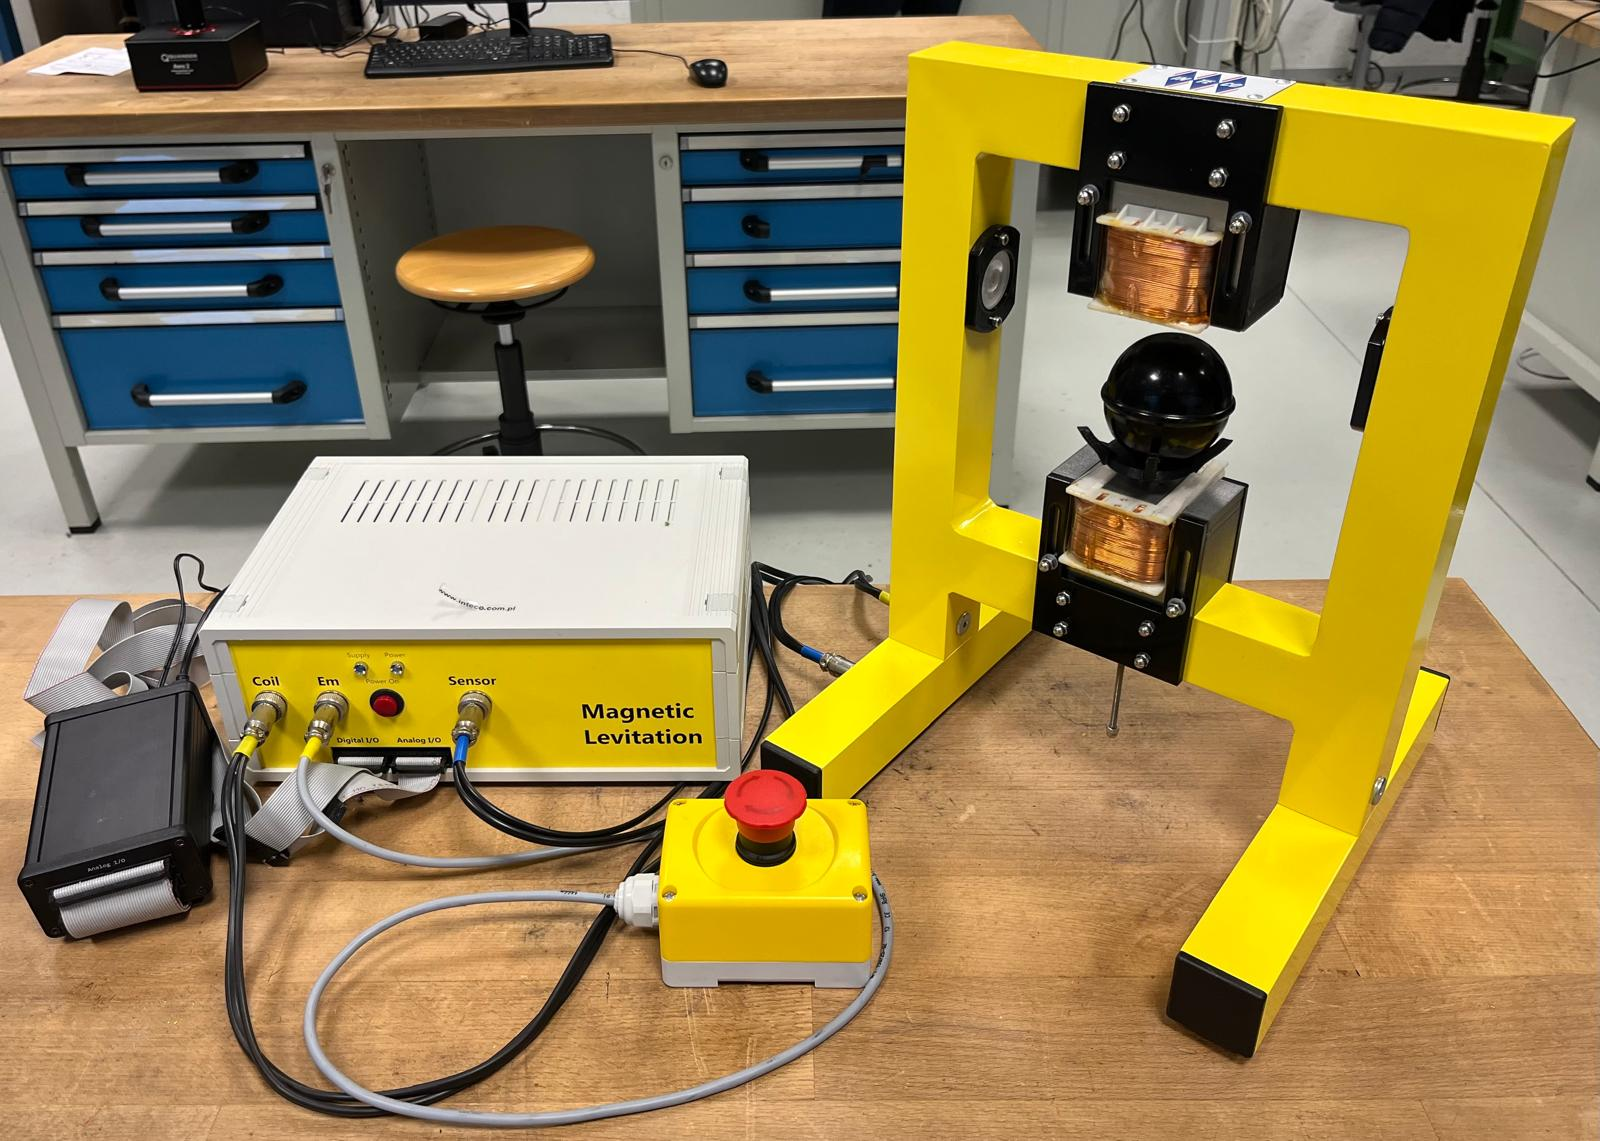
\includegraphics[width=0.7\textwidth]{./img/Maglev_from_the_lab.jpeg}
    \caption{\acrlong{mls}.}
    \label{fig:MLS}
\end{figure}

As it can be seen quite clearly, the system is composed of a simple mechanical structure that is used to support two electromagnets and an optical infrared sensor.
Along with the mechanical structure, a ferromagnetic ball and a control unit are present.

At its core principle, the system uses the interaction between the magnetic field generated by the electromagnets and the ferromagnetic ball to keep the ball in a desired position.
The optical sensor is used to measure the position of the ball and provide feedback to the control unit that, in turn, adjusts the voltage applied to (and indeed the current flowing through) the electromagnets to keep the ball in a desired position.
In Figure \ref{fig:MLS_general_scheme} a schematic representation of the upper half of the system is shown.

\begin{figure}[H]
    \centering
    \includegraphics[width=0.45\textwidth]{./img/magLev_general_scheme.png}
    \caption{A schematic representation of \acrshort{mls} is shown. One might also appreciate the feedback loop that is closed by the optical sensor. Credit to \cite{Jastrzębski2024}.}
    \label{fig:MLS_general_scheme}
\end{figure}

\paragraph{Real world application}

Magnetic levitation systems have diverse and transformative applications across various industries.

One of the most prominent uses is in high-speed transportation, such as MagLev trains, which achieve speeds exceeding $500 km/h$ by eliminating wheel-rail friction.
These systems offer smoother rides, reduced noise, and lower maintenance costs compared to traditional trains.
Notable implementations include Japan's Chūō Shinkansen (see Figure \ref{fig:mls_applications}a), aiming to connect Tokyo and Osaka, and China's $600 km/h$ MagLev project, which demonstrates cutting-edge levitation control technology \cite{WikiSCMaglev}.

Other applications include microrobotics research, where magnetic levitation enables precise control of miniature robots for possible medical and industrial applications \cite{microrobotsControl}.
These robots can navigate complex environments, perform delicate tasks, and deliver targeted therapies with high precision and minimal invasiveness.
Researchers are also exploring complex magnetic levitation environments for concurrent control of multiple robots, which could revolutionize microscale manufacturing and healthcare \cite{Independent3DControl}.

Additionally, scientific research benefits from these systems in experiments requiring vibration-free environments, such as advanced spectroscopy \cite{spectroscopy} and microgravity simulation \cite{microgravity}.


\begin{figure}[H]
    \centering
    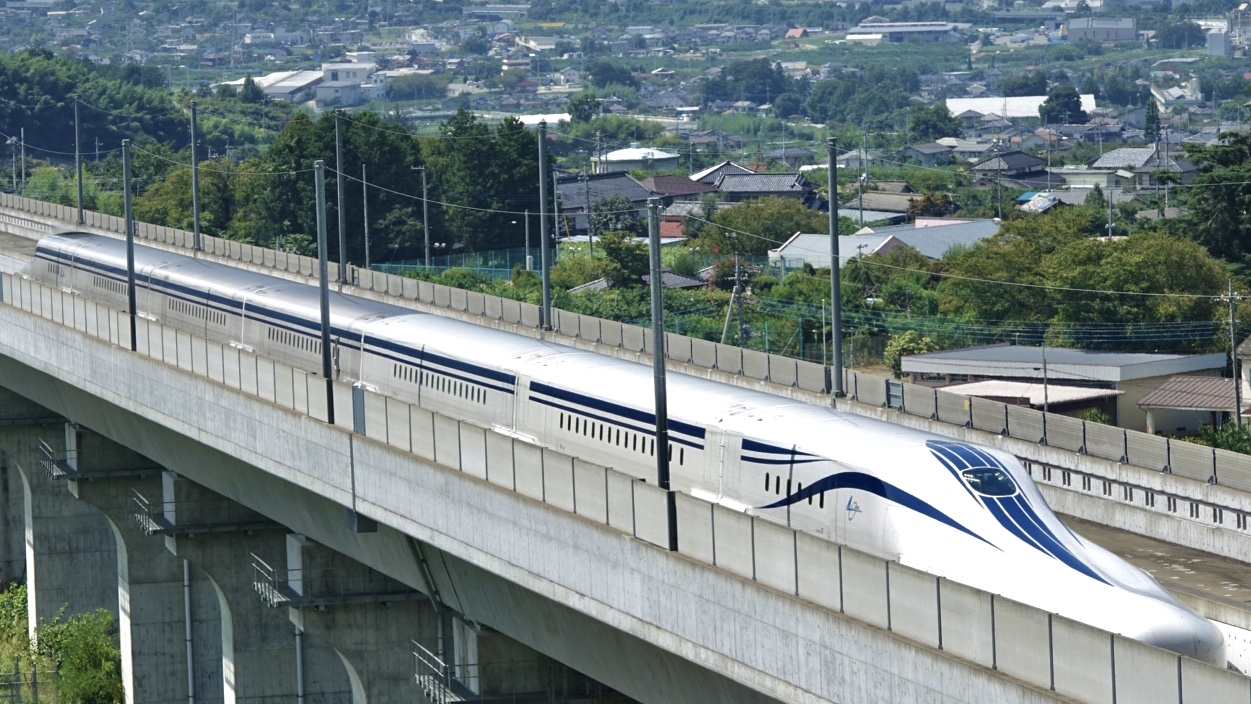
\includegraphics[height=130px]{./img/Chuo_Shinkansen.jpg}
    \hspace{1cm}
    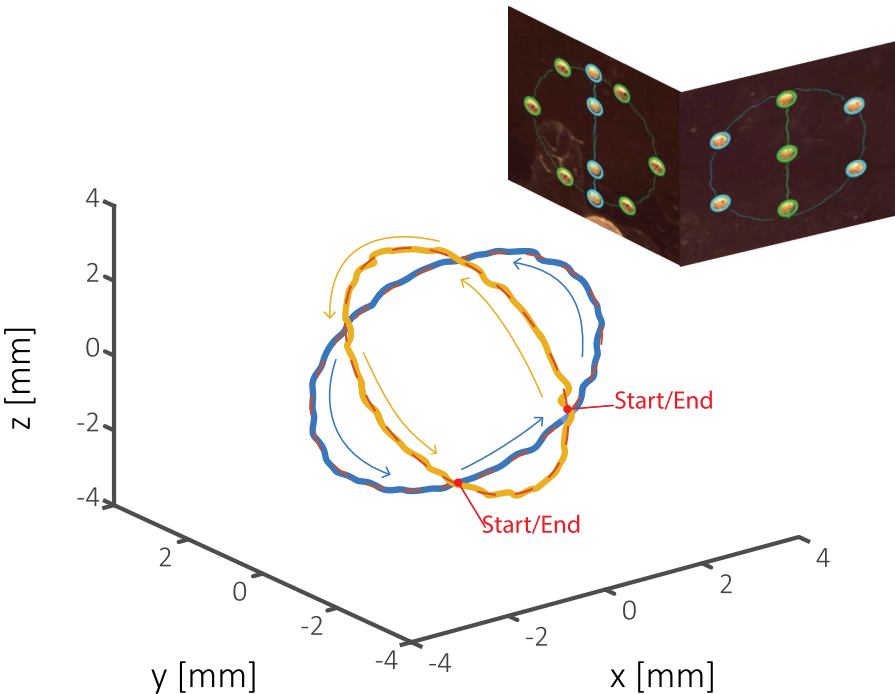
\includegraphics[height=130px]{./img/3D_magnetic_dual_control.png}
    \caption{
        Applications of Magnetic Levitation.
        Japan's MagLev train Chūō Shinkansen \cite{WikiSCMaglev} on the left, independent 3D control of a pair of microrobots via MLS techniques \cite{Independent3DControl} on the right.
    }
    \label{fig:mls_applications}
\end{figure}
